\documentclass{beamer}

\usepackage[utf8]{inputenc}
\usepackage{ae,aecompl}
\usepackage{amsfonts}
\usepackage{mathtools}
\usepackage{listings}
\usepackage{graphicx}

\begin{document}
\begin{frame}
  \frametitle{Fallout: Shelter}
  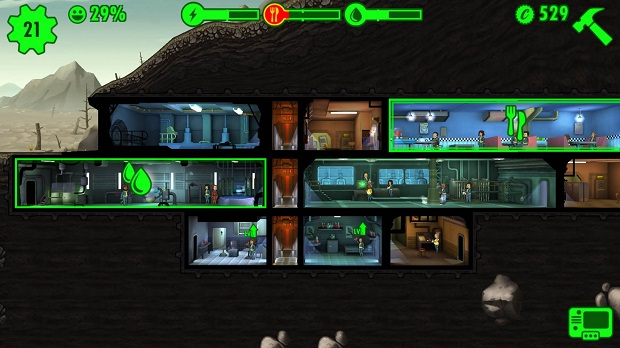
\includegraphics[width=10cm]{Fallout_Shelter_gameplay}
\end{frame}

\begin{frame}
  \frametitle{Fallout: Shelter}
  \begin{itemize}
  \item Postapocalyptic mobile game
  \item You control a shelter full of dwellers
  \item One thing dwellers can do is scout
  \item Scouts retrieve bottlecaps and items
  \item Scouts face deadly challenges
  \end{itemize}
\end{frame}


\begin{frame}
  \frametitle{SPECIAL}

{\Large \underline{Seven stats determine success}}
  \begin{itemize}
  \item Strength
  \item Perception 
  \item Endurance 
  \item Charisma 
  \item Intelligence 
  \item Agility 
  \item Luck 
  \end{itemize}
\end{frame}


\begin{frame}
  \frametitle{Retrieval: Intro}
  \begin{itemize}
  \item We wanted to know what determined how fast a scout found items and bottlecaps
  \item We performed a linear analysis and looked at the p-values
  \item The goal is to figure out if some dwellers are better scouts than others
  \end{itemize}

\end{frame}

\begin{frame}
  \frametitle{Retrieval: Items}
  \begin{table}
\caption{Number of items per hour}
\label{table:n.items}
\begin{tabular}{l|lllll}
&Estimate Std.&Error&t value&Pr(>|t|) &\\ 
\hline
(Intercept)&1.290960 &0.771921 &1.672&0.0959&.\\
level&-0.021353  & 0.017178 & -1.243 &  0.2152&  \\
dmg&-0.060882  & 0.057463 & -1.059 &  0.2906&  \\
s&-0.003986  & 0.055532 & -0.072  & 0.9428&  \\
p&-0.079242 &  0.095350 & -0.831 &  0.4069 & \\
e&0.031539 &  0.070731 &  0.446  & 0.6561&  \\
c& -0.057148  & 0.091382 & -0.625 &  0.5324&  \\
i&0.324587&0.335993&   0.966&   0.3351&  \\
a&0.214665&0.133610 &  1.607&   0.1096&  \\
l&0.042945&0.073570&0.584&0.5600&\\
\hline
\end{tabular}
\end{table}
\end{frame}


\begin{frame}
  \frametitle{Retrieval: Bottlecaps}
  \begin{table}
\caption{Average number of caps per hour}
\label{table:caps}
\begin{tabular}{l|lllll}
&Estimate&t value&Pr(>|t|)&\\  
\hline  
(Intercept)&83.81787937  &  11.63356 &<2e-162& ***\\
s &-0.21649106   & -0.43309 &    0.665802 &   \\
p&  0.61211724    & 0.91113 &   0.364235 &   \\
e & -0.88781188    &-1.67151 &   0.097489 &  . \\
c&-0.18453188  &  -0.31035  &  0.756888 &   \\
i& 0.19836365    & 0.35132  &  0.726024 &   \\
a  & -0.04815488  & -0.08799 &   0.930043&    \\
l &   13.48815469   & 26.55579&  <2e-16& ***\\
start.level &  -0.68088744   &  -4.25171 &   0.00004495 & *** \\ 
start.damage& -1.56703535   & -1.97083 &   0.051278 & . \\ 
level.increase & -3.44085855  & -1.97599 &   0.050683 &.  \\ 
death.damage & 0.30906873   &  0.88693  &  0.377067&\\
\hline
\end{tabular}
\end{table}
\end{frame}


\begin{frame}
  \frametitle{Retrieval: Conclusions}
  \begin{itemize}
  \item Difficult to determine what affects items found. Two p-values stand out, but are still bad.
    \begin{itemize}
    \item Intercept has p-value $0.96$
    \item Agility has p-value $1.1$
    \end{itemize}
  \item Caps found clearly determined by Luck (infinitesimal p-value). There's also a base value (intercept). There is also a small but clear negative correlation with level, hard to tell why this is.
  \end{itemize}
\end{frame}


\begin{frame}
  \frametitle{Survival: Intro}
  \begin{itemize}
  \item Scouts face a variety of threats.
  \item Threats can deal damage both as lost hit points and radiation, too much of either results in death.
  \item Death is nonpermanent but expensive.
  \item By calculating the expected time of death for a scout we can choose how long we dare to let our scouts roam.
  \end{itemize}
\end{frame}


\begin{frame}
  \frametitle{Survival: P-values}
  \begin{table}[]
    \centering
    \caption{Survival time}
    \label{table:survival.time}
    \begin{tabular}{l|lllll}
      &t value&Pr(>|t|)& \\ 
      \hline
      (Intercept)    &  -1.7983755246 & 0.074911&. \\ 
      s              &  2.4166724012  & 0.017339 &*\\
      p              &  0.9644124169  & 0.336994 &\\
      e              &  7.6484812878  & 9e-11&*** \\
      c              &  0.6092526555  & 0.543637& \\
      i              &  1.9626433352  & 0.052260& .\\
      a              &  1.0647793211  & 0.289351& \\
      l              &  -5.9440869849 & 3e-7&*** \\
      start.level    &  12.3797838804 & <2e-16&*** \\
      start.damage   &  4.1308435539  & 7e-4&*** \\
      level.increase &  6.4636998849  & 3e-8 &***\\
      caps           &  6.2586709017  & 8e-8&*** \\
      death.damage   &  0.7153117136  & 0.475960&\\
      \hline
    \end{tabular}
  \end{table}
\end{frame}


\begin{frame}
  \frametitle{Survival: Models}
  \begin{itemize}
  \item The best p-values among the controllable variables belong to endurance, luck, level, and starting damage.
  \item Selected models
    \begin{itemize}
    \item Linear model over all four
    \item Polynomial models over one of the above
    \item Random forest
    \end{itemize}
  \end{itemize}
\end{frame}


\begin{frame}
  \frametitle{Survival: Performance}
  
\end{frame}


\begin{frame}
  \frametitle{Survival: Conclusions}
  
\end{frame}


\begin{frame}
  \frametitle{Questions}
  {\Huge Questions}
  \begin{itemize}
  \item Questions?
  \end{itemize}

\end{frame}

\end{document}
